% --------------------------------------
% Document Class
% --------------------------------------
\documentclass[a4paper,11pt]{article}
% --------------------------------------



% --------------------------------------
% Use Package
% --------------------------------------


\usepackage[francais]{babel}
\usepackage{ucs}
\usepackage[utf8x]{inputenc}
\usepackage[T1]{fontenc}

\usepackage{makeidx}
\usepackage{color}
\usepackage{graphicx}
\usepackage{float}
\usepackage[hidelinks]{hyperref} 
\usepackage[top=2.5cm, bottom=2.5cm, left=2.5cm, right=2.5cm]{geometry}
\usepackage{lastpage}
\usepackage{marginnote}
\usepackage{fancyhdr}
\usepackage{titlesec}
\usepackage{framed}
\usepackage{amsmath}
\usepackage{array}
\usepackage{multicol}
\usepackage{adjustbox}

% insert code
\usepackage{listings}

% define our color
\usepackage{xcolor}

% code color
\definecolor{ligthyellow}{RGB}{250,247,220}
\definecolor{darkblue}{RGB}{5,10,85}
\definecolor{ligthblue}{RGB}{1,147,128}
\definecolor{darkgreen}{RGB}{8,120,51}
\definecolor{darkred}{RGB}{160,0,0}

% other color
\definecolor{ivi}{RGB}{141,107,185}


\lstset{
    language=Scilab,
    captionpos=b,
    extendedchars=true,
    frame=lines,
    numbers=left,
    numberstyle=\tiny,
    numbersep=5pt,
    keepspaces=true,
    breaklines=true,
    showspaces=false,
    showstringspaces=false,
    breakatwhitespace=false,
    stepnumber=1,
    showtabs=false,
    tabsize=3,
    basicstyle=\small\ttfamily,
    backgroundcolor=\color{ligthyellow},
    keywordstyle=\color{ligthblue},
    morekeywords={include, printf, uchar},
    identifierstyle=\color{darkblue},
    commentstyle=\color{darkgreen},
    stringstyle=\color{darkred},
}


% --------------------------------------



% --------------------------------------
% Page setting
% --------------------------------------
%\pagestyle{empty}
\setlength{\headheight}{15pt}

\setcounter{secnumdepth}{3}
\setcounter{tocdepth}{2}

\makeatletter
\@addtoreset{chapter}{part}
\makeatother 

\hypersetup{         % parametrage des hyperliens
  colorlinks=true,      % colorise les liens
  breaklinks=true,      % permet les retours à la ligne pour les liens trop longs
  urlcolor= blue,       % couleur des hyperliens
  linkcolor= black,     % couleur des liens internes aux documents (index, figures, tableaux, equations,...)
  citecolor= green      % couleur des liens vers les references bibliographiques
}

% --------------------------------------

% --------------------------------------
% Information
% --------------------------------------
\title{Compte-rendu TP1 TI : Sources lumineuses}
\author{Elliot VANEGUE et Gaëtan DEFLANDRE}
% --------------------------------------

\definecolor{myColor}{rgb}{0.5, 0.1, 0.75}

% --------------------------------------
% Begin content
% --------------------------------------
\begin{document}

% Set language to english
  \selectlanguage{francais}

  % Start the page counting
  \pagenumbering{arabic}

  \maketitle
  
  \mbox{}
  \newpage
  \clearpage
  
  \section*{Introduction}
  Nous allons, dans ce premier TP, étudier l'éclairement de différent type
  de source lumineuse via l'outils Scilab. Le but est de trouver l'emplacement
  de plusieurs source lumineuse afin que l'éclairement d'une surface soit homogène.\\
  
  \section{Eclairement d'une source ponctuelle isotrope}
  Une source ponctuelle isotrope émet la même intensité énergétique dans toutes les 
  directions. Nous allons, donc, voir commet calculer l'éclairement d'une surface
  avec cette source.\\
  
  Nous avons modifié le code en exemple afin de calculer les valeurs d'éclairement de 
  chaque élément de la surface par une source lumineuse isotrope. Nous obtenons le code 
  suivant :
  
  \begin{lstlisting}[caption=Code Scilab eclairement source isotrope]
  
  // Definition des echantillons sur un axe
  axe = [0:99] / 100 + 5e-3;
  // Definition des elements de surface
  x = ones (1:100)' * axe;
  y = axe' * ones (1:100);
  // Position de la source -> sur le plan
  xs = 0.5;
  ys = 0.5;

  // Calcul de la distance
  d = sqrt ((x - xs).^2 + (y - ys).^2);

  // Puissance
  Phi=100;

  // Intensite energetique
  I0=Phi/2/%pi;

  // Hauteur
  h= 0.5;

  // Eclairement
  e = I0 * (h .* ((h^2 + d.^2).^(-3/2)));
  plot3d (axe, axe, e);
  imshow (e/max(e));

  \end{lstlisting}
  
  Soit le calcul de l'éclairement:
  
  $$ \Phi = 100 W $$
  $$ cos(\theta) = \frac{h}{\sqrt{h^{2}+d^{2}}} $$
  $$ E(P)=\frac{\Phi}{(h^{2}+d^{2})*2\pi}*cos(\theta) $$
  
  Avec ce calcul nous obtenons une courbe comme celle-ci :
  
  \begin{figure}[H]
    \center
    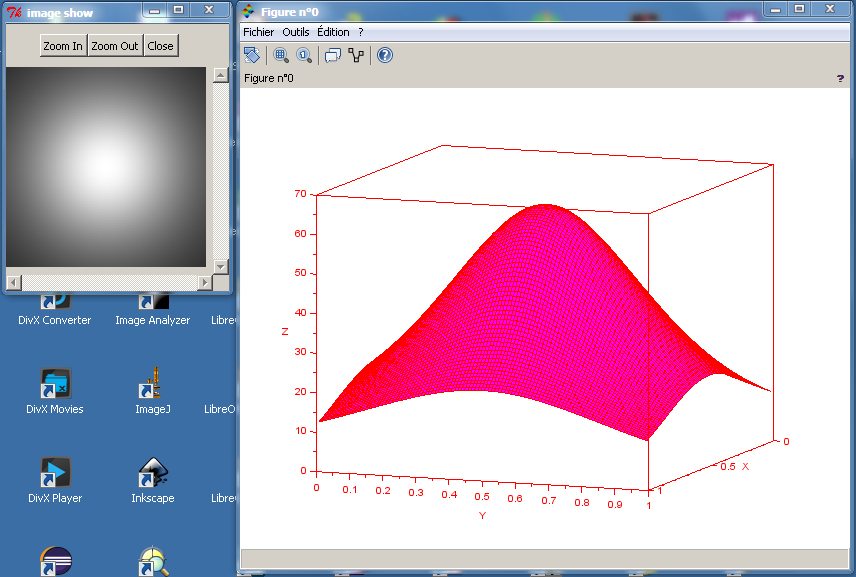
\includegraphics[width=10cm]{../isotrope.PNG}
    \caption{Graphique de la répartition de la lumière d'une source isotrope}
  \end{figure}
  
  Sur ce graphique, nous pouvons voir que la lumière est plus intense sur la surface juste
  en dessous de la source lumineuse. Puis, l'éclairement reçu par la surface diminu sur les 
  bords de la surface.

  \section{Eclairement d'une source ponctuelle lambertienne}
  Une source lambertienne adopte un schéma un peu différent d'une source ponctuelle isotrope.
  Le diagramme d'émission de cette source est fonction du cosinus de l'angle d'émission.
  
  \begin{figure}[H]
    \center
    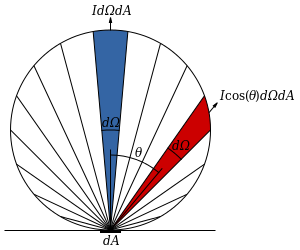
\includegraphics[width=7cm]{../Lambert_Cosine_Law_1.png}
    \caption{Représentation d'une source lumineuse isotrope lambertienne}
  \end{figure}
  
  \newpage
  
  Nous avons à nouveau modifié le code afin de prendre en compte cette dispersion de la 
  lumière. Nous obtenons le calcul suivant :
  
  \begin{lstlisting}[caption=Nouvelle eclairement pour une source lambersienne]
  // Eclairement avec source de lambert
  e = I0 * ((h^2) .* ((h^2 + d.^2).^(2)).^(-1))
  \end{lstlisting}
  
  Donc le calcul:
  
  $$ E(P)=\frac{\Phi}{(h^{2}+d^{2})*2\pi}*cos(\theta)^{2} $$\\
  
  Ici nous voyons que l'exposant du dénominateur à changé, car pour une source lambertienne, 
  le cosinus de l'angle theta intervient deux fois.
  \begin{itemize}
    \item Une première fois, comme pour la source isotrope, la source ponctuelle émet dans toute 
    les directions. Donc les rayons, avec pour direction la normale de la source arrive plus 
    directement sur la surface de l'objet. Plus l'angle par rapport à la normale de la source 
    grandit, plus la distance que les rayons devrons parcourir sera grande.
    \item Une seconde fois, car dans le cas de la source lambertienne, plus l'angle par rapport 
    à la normale augmente, plus éclairement diminu, fonction du cosinus de cette angle 
    (\textit{cf FIGURE 2}).\\
  \end{itemize}
  
  \begin{figure}[H]
    \center
    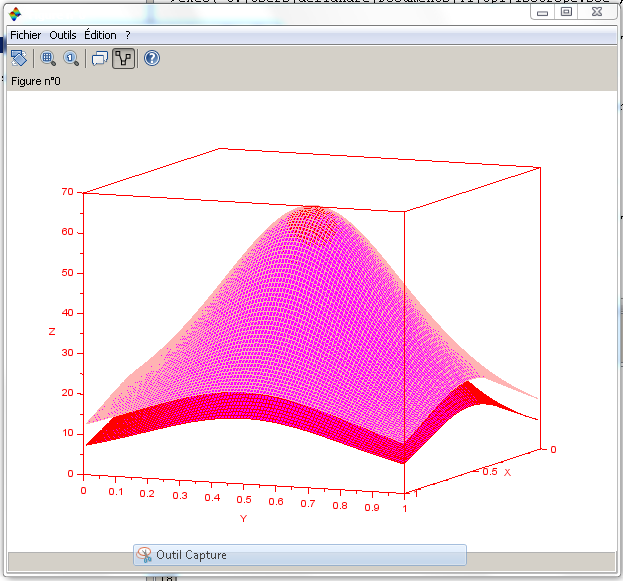
\includegraphics[width=10cm]{../iso_lamb.PNG}
    \caption{Graphique des sources ponctuelle (rose claire) et lambertienne (rose foncé)}
  \end{figure}
  
  \newpage
  
  Ce calcul nous donne une courbe avec une pente plus importante car la lumière éclaire moins
  les bords de la surface par rapport à une source ponctuelle isotrope. En effet, l'éclairement 
  d'une source de lambert décroit plus vite lorsque l'angle $\theta$ est grand.
  
  \section{Eclairement d'une grille de source ponctuelle}
  
  Nous allons, maintenant, disposer plusieurs sources lambersiennes de manière à minimiser la 
  variance quelque soit le nombre de sources. Il faut positionner sur une grille de \textbf{N*N}
  sources \textbf{régulièrement espacées}.
  
  \begin{lstlisting}[caption=Code pour l'eclairement d'une grille de sources ponctuelles]
    // TODO faire avec un carre de cote 4.
  \end{lstlisting}
  
  \section*{Conclusion}
    
\end{document}